\documentclass[tikz,border=12pt]{standalone}
\usepackage[T1]{fontenc}
\usepackage{mathpazo}
\usepackage{amsmath,amssymb}
\usetikzlibrary{arrows.meta, positioning, calc}

\definecolor{stblue}{HTML}{7B97AD}
\definecolor{rwgold}{HTML}{B8995E}
\definecolor{sage}{HTML}{7A9A7E}
\definecolor{dkbrown}{HTML}{3D3530}
\definecolor{wmgray}{HTML}{7B7067}
\definecolor{cream}{HTML}{F9F6F0}
\definecolor{border}{HTML}{D4C9B8}
\definecolor{terracotta}{HTML}{C47A6A}
\definecolor{lavender}{HTML}{907EA0}

\begin{document}
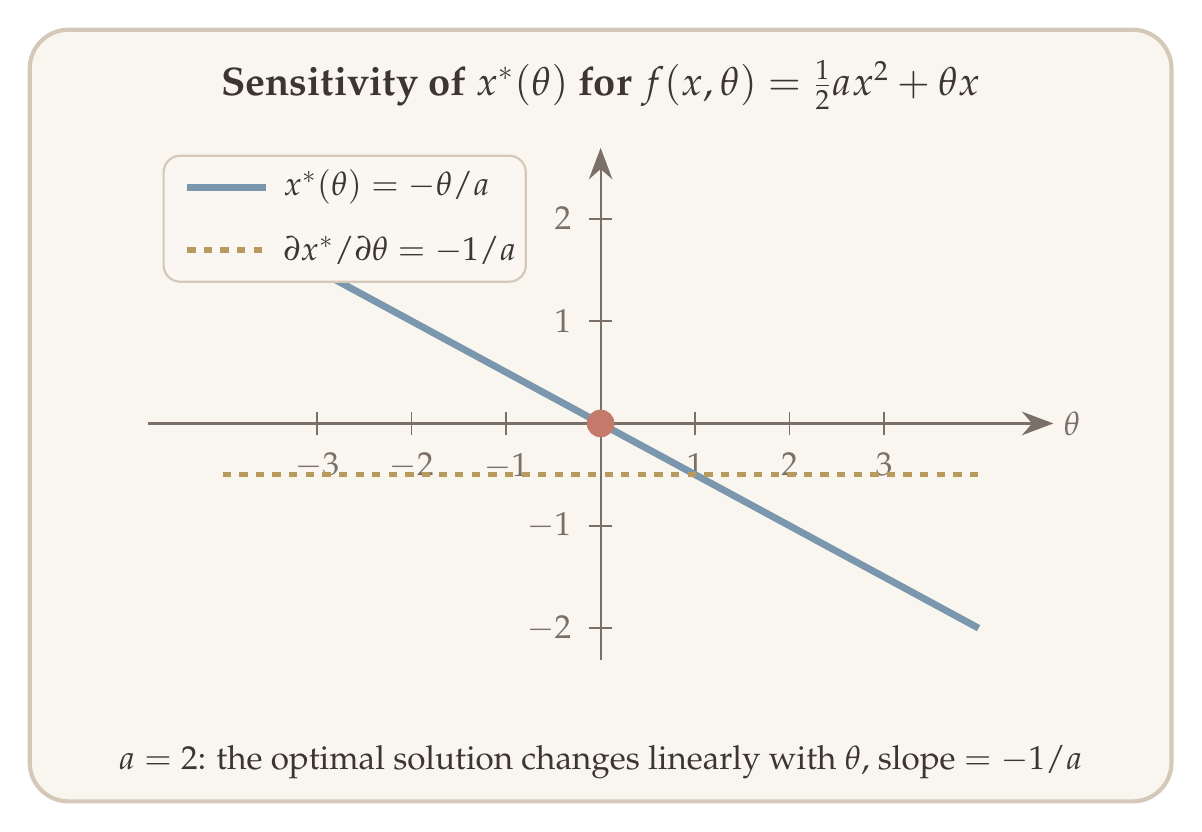
\begin{tikzpicture}[>={Stealth[length=4mm, width=3mm]}]

% Background
\fill[cream, rounded corners=14pt] (-0.5,-0.8) rectangle (14,9);
\draw[border, line width=1.5pt, rounded corners=14pt] (-0.5,-0.8) rectangle (14,9);

% Title
\node[text=dkbrown, font=\Large\bfseries] at (6.75,8.3)
  {Sensitivity of $x^*(\theta)$ for $f(x,\theta) = \tfrac{1}{2}ax^2 + \theta x$};

% Coordinate mapping:
% theta-range: -4 to 4, center at canvas x=6.75
% y-range: -2.5 to 2.5, center at canvas y=4.0
% x-scale: 1.2, y-scale: 1.3

% Axes
\draw[wmgray, line width=0.8pt, ->] (1.0,4.0) -- (12.5,4.0)
  node[right, font=\large, text=wmgray] {$\theta$};
\draw[wmgray, line width=0.8pt, ->] (6.75,1.0) -- (6.75,7.5)
  node[above, font=\large, text=wmgray] {};

% theta -> 6.75 + theta*1.2
% y -> 4.0 + y*1.3

% Tick marks theta-axis
\foreach \t/\lab in {-3/-3, -2/-2, -1/-1, 1/1, 2/2, 3/3} {
  \draw[wmgray, line width=0.6pt] ({6.75+\t*1.2},3.85) -- ({6.75+\t*1.2},4.15);
  \node[text=wmgray, font=\large, below] at ({6.75+\t*1.2},3.75) {$\lab$};
}

% Y-axis ticks
\foreach \v/\lab in {-2/-2, -1/-1, 1/1, 2/2} {
  \draw[wmgray, line width=0.6pt] (6.6,{4.0+\v*1.3}) -- (6.9,{4.0+\v*1.3});
  \node[text=wmgray, font=\large, left] at (6.5,{4.0+\v*1.3}) {$\lab$};
}

% x*(theta) = -theta/a with a=2, so slope = -1/2
% Line from theta=-4 to theta=4: y = -theta/2
% theta=-4: y=2, canvas (1.95, 6.6)
% theta=4: y=-2, canvas (11.55, 1.4)
\draw[stblue, line width=2.5pt] (1.95, 6.6) -- (11.55, 1.4);

% dx*/dtheta = -1/a = -0.5, constant
% Horizontal dashed line at y = -0.5
% canvas y = 4.0 + (-0.5)*1.3 = 3.35
\draw[rwgold, line width=2pt, dashed] (1.95, 3.35) -- (11.55, 3.35);

% Origin marker
\fill[terracotta] (6.75,4.0) circle (5pt);

% Legend
\fill[cream!90!white, rounded corners=6pt] (1.2,5.8) rectangle (5.8,7.4);
\draw[border, line width=0.8pt, rounded corners=6pt] (1.2,5.8) rectangle (5.8,7.4);
\draw[stblue, line width=2.5pt] (1.5,7.0) -- (2.5,7.0);
\node[text=dkbrown, font=\large, right] at (2.6,7.0) {$x^*(\theta) = -\theta/a$};
\draw[rwgold, line width=2pt, dashed] (1.5,6.2) -- (2.5,6.2);
\node[text=dkbrown, font=\large, right] at (2.6,6.2) {$\partial x^*/\partial\theta = -1/a$};

% Annotation
\node[text=dkbrown, font=\large] at (6.75,-0.3)
  {$a = 2$: the optimal solution changes linearly with $\theta$, slope $= -1/a$};

\end{tikzpicture}
\end{document}
